\addcontentsline{toc}{section}{CAPÍTULO VII}
\chapter{ARQUITECTURA DE LA SOLUCIÓN}

\section{Visión general: \textit{pipeline} de dos fases}

La arquitectura de \textbf{NexusCare} cambió respecto al prototipo de Capstone 1. El prototipo utilizaba un único modelo (MedGemma-4B) para analizar la liquidación completa. El sistema de Capstone 2 separa el procesamiento en dos fases independientes:

\begin{itemize}
    \item \textbf{Fase 1:}  motor de reglas contractuales determinístico (sin IA). Verifica elegibilidad, exclusiones y coberturas contra la configuración del plan de salud.
    \item \textbf{Fase 2:}  evaluación clínica con LLM. Analiza la consistencia clínica del expediente y genera puntajes de riesgo con justificaciones textuales.
\end{itemize}

¿Por qué separar en dos fases? Porque la Fase 1 filtra cerca del 25 \% de los ítems de cada liquidación como excluidos o condicionales, sin invocar ningún modelo de lenguaje, lo que reduce el costo de API y la latencia. Además, una exclusión contractual es determinista y verificable, a diferencia de una inferencia probabilística del LLM.

El \textit{pipeline} completo sigue un flujo secuencial: Anonimización, Fase 1, \textit{Routing}, Fase 2, Decisión. Lo orquesta el módulo orchestrator.py, que gestiona errores, \textit{logging} y estimación de costos.

El diagrama se presenta en la Figura~\ref{fig:p23_figure_1} el diagrama de contexto~\ref{fig:p24_figure_1} y diagrama de contenedores~\ref{fig:p25_figure_1}

\begin{figure}[H]
\centering
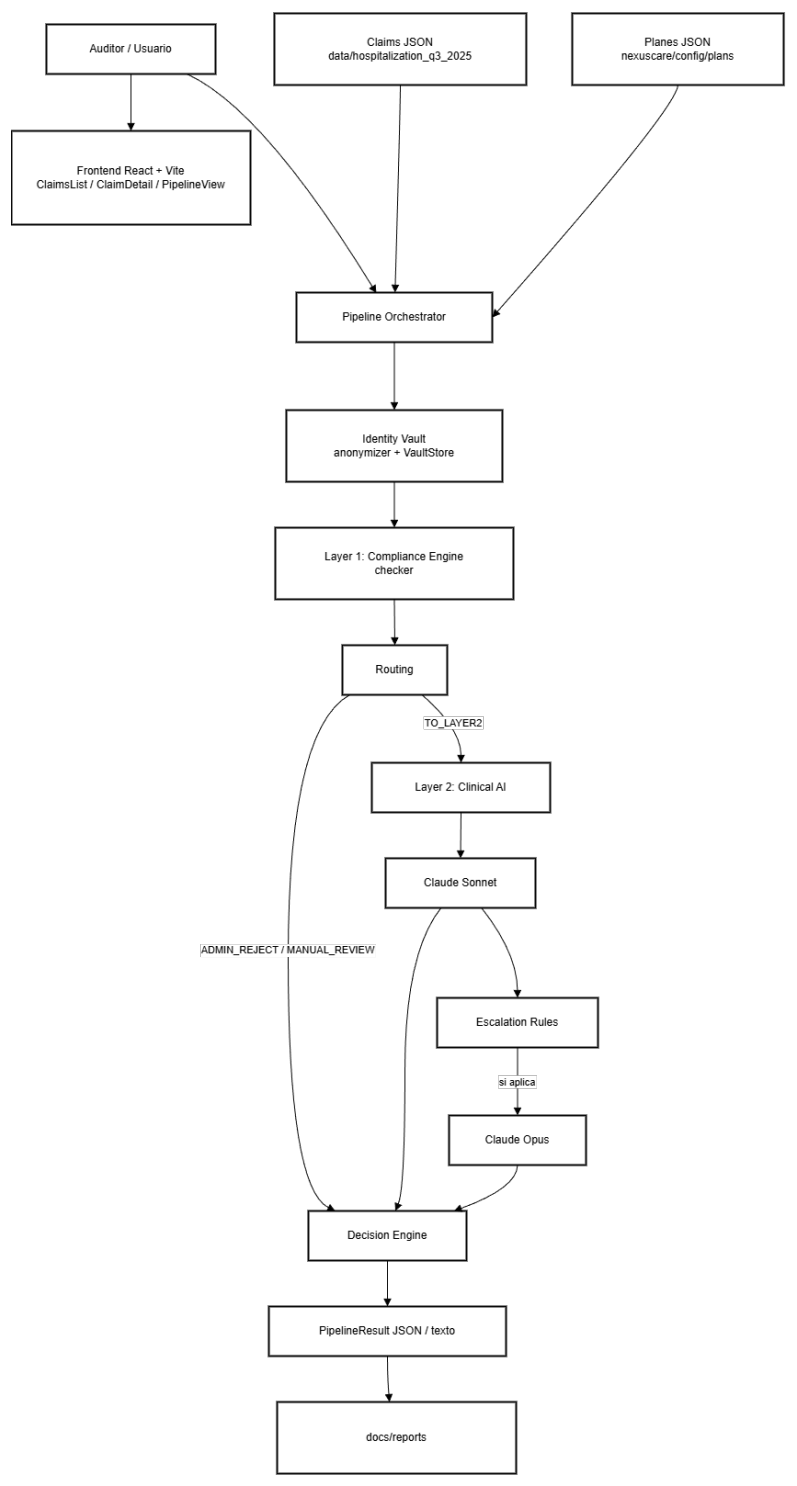
\includegraphics[width=0.96\textwidth,height=0.72\textheight,keepaspectratio]{images/p23_figure_1.png}
\caption{\textit{Workflow} del sistema: flujo de cinco fases desde la liquidación hasta la decisión del auditor.}
\label{fig:p23_figure_1}
\end{figure}

\begin{figure}[H]
\centering
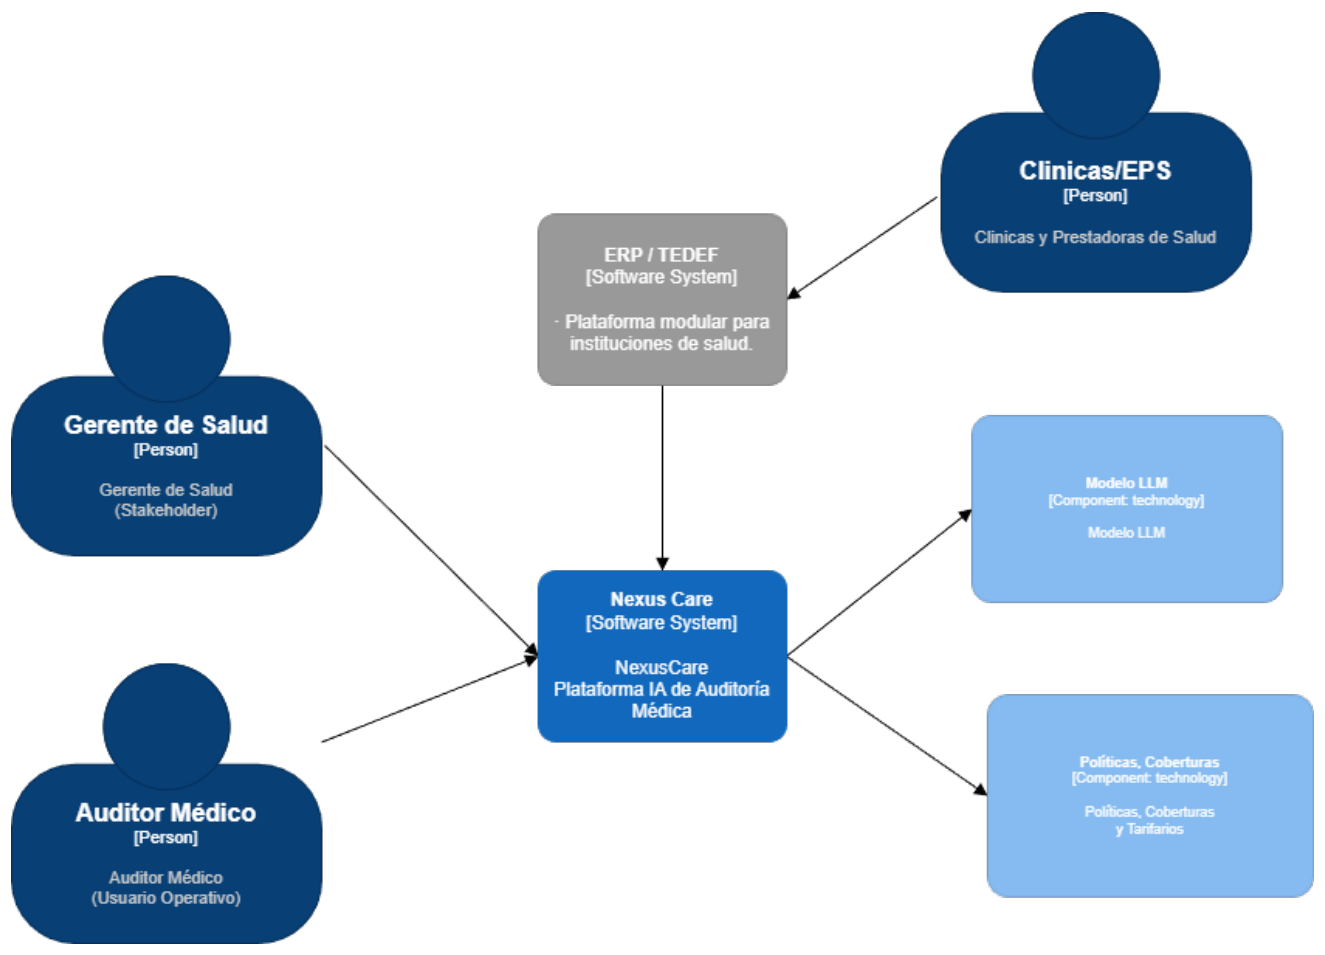
\includegraphics[width=0.96\textwidth,height=0.72\textheight,keepaspectratio]{images/p24_figure_1.png}
\caption{Diagrama C4 de contexto del problema: nivel 1 \cite{brown2018c4}.}
\label{fig:p24_figure_1}
\end{figure}

\begin{figure}[H]
\centering
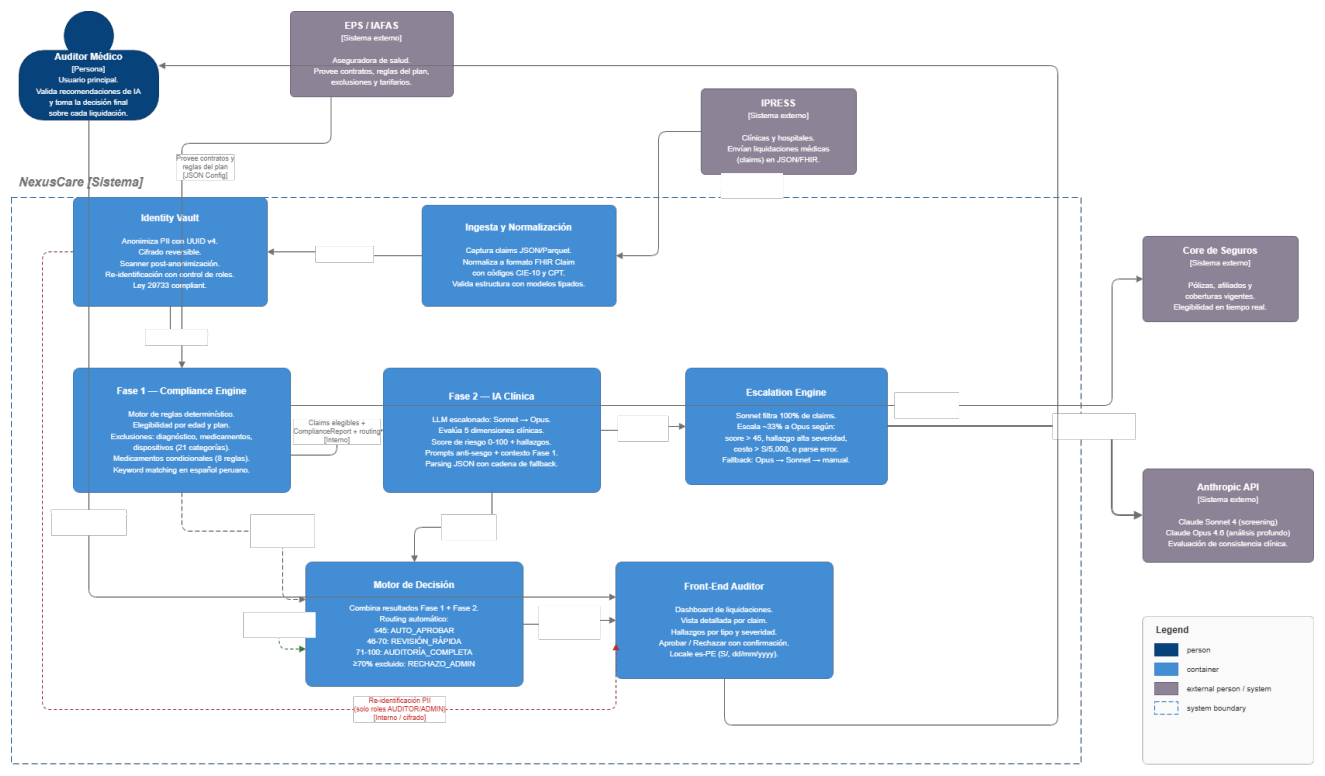
\includegraphics[width=0.96\textwidth,height=0.72\textheight,keepaspectratio]{images/p25_figure_1.png}
\caption{Diagrama C4 de contenedores del sistema.}
\label{fig:p25_figure_1}
\end{figure}

\section{Ingesta y normalización}

Las liquidaciones llegan como archivos JSON individuales, cada uno representando un caso hospitalario completo. La estructura incluye:
\begin{itemize}
     \item \textbf{Datos del paciente:}  nombre, edad, sexo (los dos últimos se preservan como quasi-identificadores necesarios para la validación clínica CIE-10).

     \item \textbf{Datos del prestador:} nombre del médico tratante (anonimizado) y especialidad.

    \item \textbf{Diagnóstico:} código CIE-10 y descripción textual.

    \item \textbf{Servicios:} organizados en siete categorías (farmacia, procedimientos, clínica, imagenología, consultas, laboratorio, otros servicios), cada una con una lista de ítems que incluyen código, descripción y costo.
     
\end{itemize}

La validación estructural se realiza mediante modelos Pydantic v2, definidos en nexuscare/compliance/models.py.

La clase \textit{Claim} y sus modelos anidados garantizan que toda liquidación procesada cumpla con el esquema esperado. Los principales modelos involucrados son Patient, Provider, Diagnosis, Services, ServiceCategory y ServiceItem.

Los costos se almacenan como strings para preservar el formato original y se convierten a float bajo demanda mediante la propiedad cost float de ServiceItem.

La fuente de datos del MVP consiste en 101 liquidaciones hospitalarias del Q3 2025 de MediVida, complementadas con registros proxy de pacientes (visitas únicas y múltiples) indexados por un catálogo maestro (patient index.json).

\section{\textit{Identity Vault}: protección de datos personales}

Antes de que cualquier dato llegue al LLM, el sistema ejecuta un proceso de anonimización que implementa los principios de \textit{privacy} by design establecidos en Capstone 1 \cite{hurtado2025nexuscare}, en cumplimiento con la Ley No 29733 \cite{peru2011ley29733} y alineado con los principios de minimización de datos del GDPR \cite{eu2024aiact}.

El módulo \textit{Identity Vault} (nexuscare/vault/) comprende cuatro componentes:

 \textbf{\textit{Anonymizer} (anonymizer.py)} Reemplaza los nombres de paciente y médico con identificadores UUID v4. El proceso es idempotente: la misma persona siempre recibe el mismo UUID, lo que permite correlacionar liquidaciones de un mismo paciente sin exponer su identidad. Los datos clínicos (diagnósticos, medicamentos, costos) no se anonimizan porque son necesarios para el análisis de consistencia.

 
 \textbf{\textit{Scanner} (scanner.py)} Detector de fugas de PII post-anonimización. Busca patrones específicos del contexto peruano: DNI (8 dígitos), números CMP (Colegio Médico del Perú), números
 \textbf{\textit{Vault Store} (store.py)} Almacenamiento persistente cifrado para los mapeos PII-UUID. Utiliza AES-256-GCM con derivación de clave mediante SHA-256 sobre la clave de entorno (VAULT\_KEY). Mantiene dos índices: anon\_id hacia PIIRecord (para re-identificación) y \textit{hash} del \textit{lookup key} hacia anon id (para anonimización idempotente).
telefónicos con prefijo +51, y direcciones de correo electrónico. Los UUID se excluyen del escaneo porque son valores esperados en datos anonimizados.

\textbf{\textit{Reidentifier} (reidentifier.py)} Servicio de re-identificación con control de acceso basado en roles. Solo los roles AUDITOR y ADMIN pueden resolver un UUID a la identidad real. Cada operación de re-identificación se registra en un log de auditoría inmutable (\textit{append-only}), cumpliendo el requisito de trazabilidad (RF5).

El flujo completo es: \textit{Claim}(PII) → Anonymize → \textit{Claim}(anon) → LLM → Result → Re-identify → Auditor. En ningún momento el LLM procesa datos que permitan identificar a un paciente o médico real.

\section{Fase 1: motor de reglas contractuales}

Fase 1 implementa la verificación determinística de cumplimiento contractual. Es la primera línea de filtrado y opera sin ningún componente de IA.

El motor está implementado en nexuscare/compliance/ y ejecuta cinco verificaciones secuenciales sobre cada liquidación:

\noindent \textbf{1. Elegibilidad por edad} Verifica que la edad del paciente se encuentre dentro del rango de ingreso permitido por el plan. Para MediVida Más 65, el rango es de 65 a 100 años; para MediVida Premium, de 0 a 64 años. Un paciente fuera del rango de su plan genera un \textit{finding EXCLUDED} en la categoría \textit{eligibility} y el \textit{claim} se envía a AUDITORIA COMPLETA, sin pasar por el LLM.

\noindent \textbf{2. Validación de diagnóstico} CIE-10 Consulta un catálogo CIE-10 embebido para verificar: (a) que el código diagnóstico existe, (b) que es consistente con el sexo del paciente, y (c) que es consistente con el rango de edad. Este módulo (cie10.py) realiza una búsqueda fuzzy para manejar variaciones en la codificación.


\noindent \textbf{3. Exclusiones por diagnóstico} Evalúa 21 exclusiones generales definidas en la configuración del plan, cada una con sus prefijos CIE-10 asociados. Las categorías incluyen: enfermedades congénitas (prefijo Q), accidentes laborales (Z57), deportes de riesgo (V, W, X, Y), abuso de sustancias (F10–F19, T40–T51), salud mental (F), cirugía estética y tratamientos de obesidad, entre otras. Algunas exclusiones tienen excepciones textuales que se preservan como \textit{findings} de tipo REVIEW\_NEEDED.
\noindent \textbf{4. Exclusiones de medicamentos} Verifica cada ítem de la farmacia contra 25 categorías de medicamentos excluidos (anticonceptivos, vitaminas, psicotrópicos, hormonoterapia, etc.) mediante \textit{keyword matching} con normalización de texto en español. También evalúa 8 medicamentos condicionales cuya cobertura depende del diagnóstico.

\noindent \textbf{5. Exclusiones de dispositivos e implantes} Verifica 26 \textit{keywords} de exclusión (prótesis, stents, marcapasos, etc.) frente a 37 \textit{keywords} de excepción (stents coronarios, placas y tornillos de traumatología, válvulas de derivación, etc.). La lógica distingue entre insumos médicos básicos y dispositivos que requieren verificación contractual.

La normalización de texto en español (matchers.py) maneja tildes, caracteres especiales y mayúsculas de forma consistente. Esto es necesario porque las descripciones de medicamentos e insumos en las liquidaciones peruanas emplean convenciones de escritura heterogéneas.

Las configuraciones de plan se extraen de los contratos de seguro reales en formato PDF utilizando un proceso semiautomático: un LLM genera una primera versión JSON a partir de secciones específicas del contrato (extract plan rules.py), y un auditor humano valida y corrige el resultado (validate extraction.py). Los archivos JSON resultantes se almacenan en nexuscare/config/plans/ y se versionan junto con el código.

\textbf{\textit{Routing} de Fase 1} El resultado de Fase 1 determina el siguiente paso:
\begin{itemize}
    \item Si el paciente no es elegible: AUDITORIA_COMPLETA (omite LLM).
    \item Si el 70 \% o más de los ítems están excluidos: RECHAZO_ADMINISTRATIVO (omite LLM).
    \item  En cualquier otro caso: TO_LAYER2 (envía a Fase 2 para evaluación clínica).
\end{itemize}

Este \textit{routing} permite ahorrar el costo del LLM cuando ya existe una determinación contractual clara.

\section{Fase 2: evaluación clínica con LLM}

La Fase 2 es el componente de inteligencia artificial del \textit{pipeline}. Evalúa la consistencia clínica del expediente y asigna un puntaje de riesgo explicable.

\textbf{Evolución desde Capstone 1} El prototipo usaba MedGemma-4B, un modelo de fundación médica de Google DeepMind \cite{google2025medgemma}, desplegado localmente. Los resultados fueron alentadores (93 \% de \textit{parsing} exitoso), pero el modelo presentaba limitaciones: un contexto de 8,192 \textit{tokens} insuficiente para liquidaciones con más de 100 ítems, y una tendencia a producir análisis superficiales en casos complejos.

Para Capstone 2, se realizó un \textit{benchmark} comparativo Tabla~\ref{tab:benchmark-modelos-fase2} de cinco modelos sobre las 101 liquidaciones del \textit{dataset}  (505 evaluaciones totales):

\begin{table}[H]
    \centering
    \caption{Benchmark comparativo de modelos para la Fase 2}
    \label{tab:benchmark-modelos-fase2}

    \footnotesize
    \setlength{\tabcolsep}{5pt}
    \renewcommand{\arraystretch}{1.2}

    \begin{tabular}{
        l
        c
        c
        c
        c
        c
    }
        \toprule
        \textbf{Modelo}
        & \shortstack{\textbf{\textit{Sigma score}}}
        & \textbf{Hallazgos/caso}
        & \shortstack{\textbf{Costo/caso}\\\textbf{(USD)}}
        & \shortstack{\textbf{Fast-track}\\\textbf{(\%)}}
        & \shortstack{\textbf{Latencia}\\\textbf{promedio}} \\
        \midrule

        Claude Sonnet 4 & 20.1 & 3.0 & USD 0.028 & 24.8\,\% & $\sim 17$ s \\
        Claude Opus 4.6 & 15.3 & 6.8 & USD 0.278 & 3.1\,\%  & $\sim 50$ s \\
        GPT-5.4          & 8.8  & 6.2 & USD 0.027 & 0.0\,\%  & $\sim 27$ s \\
        Gemini 2.5 Pro   & 12.2 & 3.5 & USD 0.018 & 1.0\,\%  & $\sim 38$ s \\
        MedGemma 27B     & 14.7 & 2.9 & USD 0.041 & 2.0\,\%  & Variable \\

        \bottomrule
    \end{tabular}
\end{table}

La desviación estándar del puntaje (\textit{sigma score}) mide la capacidad de discriminación del modelo: un sigma alto indica que el modelo diferencia entre casos de bajo y alto riesgo, mientras que un sigma bajo indica que asigna puntajes similares a todos los casos. Claude Sonnet 4 presentó la mayor discriminación ($\sigma$ = 20.1), con una distribución equilibrada entre las tres bandas de riesgo (25 \% bajo / 45 \% medio / 31 \% alto). GPT-5.4, con $\sigma$ = 8.8, asignó puntajes altos a prácticamente todas las liquidaciones (0 \% de \textit{fast-track}), lo que lo hace inviable para el caso de uso.

Claude Opus 4.6 generó el análisis clínico más profundo (6.8 hallazgos por caso, 682 totales), pero a un costo 10 veces mayor que Sonnet y con una tasa de \textit{fast-track} del 3.1 \%, lo que refleja una tendencia a sobrevalorar el riesgo.

Estos resultados motivaron la adopción de una estrategia escalonada, implementada en nexuscare/pipeline/escalate

\textbf{Paso 1:} Claude Sonnet 4 filtra el 100 \% de las liquidaciones ($\sim$17 segundos, \$0.028 por caso).

\textbf{Paso 2:} Se escala a Claude Opus 4.6 el $\sim$33 \% de los casos, según cuatro criterios: (a) puntaje de Sonnet > 45, (b) hallazgo de alta severidad de tipo inconsistencia clínica o sobrecosto, (c) costo total de la liquidación > S/5,000 con ítems en revisión, o (d) error de \textit{parsing} en la respuesta de Sonnet.

\textbf{\textit{Fallback}:} si Opus falla (error de parseo o \textit{timeout}), el sistema revierte al resultado de Sonnet.

El costo por liquidación con la estrategia escalonada es de $\sim$\$0.12, un 57 \% inferior al costo de usar Opus en todos los casos (\$0.278). Para un lote de 101 liquidaciones, el costo total de API fue de \$12.00, frente a \$28.08 con Opus en exclusiva.

\textbf{Ejemplo ilustrativo del benchmark} La liquidación H0710170 (obstrucción del conducto biliar, K83.1, 118 ítems, gastroenterología) fue evaluada por los cinco modelos. Claude Sonnet le asignó un puntaje de 70 e identificó 3 hallazgos. Claude Opus le asignó 75 puntos con 7 hallazgos, detectando la duplicidad terapéutica de inhibidores de bomba de protones y un patrón de reversiones en farmacia que sugiere problemas de control de inventario. Todos coincidieron en la inconsistencia principal: material endoscópico presente sin un procedimiento endoscópico registrado. Esta convergencia en el hallazgo principal, con divergencia en la profundidad del análisis complementario, justifica la estrategia escalonada.

\textbf{Dimensiones de evaluación clínica} El LLM evalúa cada liquidación en cinco dimensiones, definidas en el \textit{prompt} de auditoría (nexuscare/benchmark/prompts.py):

\noindent \textbf{1. Consistencia diagnóstico-procedimiento.}

\noindent \textbf{2. Consistencia diagnóstico-especialidad.}

\noindent \textbf{3. Protocolo farmacológico.}

\noindent \textbf{4. Materiales e insumos.}

\noindent \textbf{5. Puntaje de riesgo (0–100).}

La escala de producción utiliza cuatro bandas calibradas con el \textit{Golden Set}: 0–25 muy bajo, 26–45 bajo, 46–70 medio, 71–100 alto. Los hallazgos se tipifican en cuatro categorías: \textbf{Inconsistencia Clínica, Omisión, Sobrecosto y Duplicado.} Cada hallazgo lleva una severidad (alta, media, baja).

La salida del LLM se estructura como JSON con campos tipados, lo que permite al \textit{pipeline} procesarla de forma programática. El módulo de \textit{parsing} (extract json en run benchmark.py) maneja respuestas con bloques de código en \textit{Markdown}. Cuando el \textit{parsing} falla, el caso se marca como \textit{parse error} y se escala a Opus o se deriva a auditoría completa.

\section{Motor de decisión y \textit{routing}}

El módulo nexuscare/pipeline/decision.py combina los resultados de Fase 1 y Fase 2 para generar la recomendación final. Las reglas de decisión se encuentran en la Tabla~\ref{tab:reglas-decision-pipeline}:

\begin{table}[H]
    \centering
    \caption{Reglas de decisión del \textit{pipeline} integrado}
    \label{tab:reglas-decision-pipeline}

    \footnotesize
    \setlength{\tabcolsep}{8pt}
    \renewcommand{\arraystretch}{1.2}

    \begin{tabular}{
        p{0.62\textwidth}
        p{0.30\textwidth}
    }
        \toprule
        \textbf{Condición}
        & \textbf{Decisión} \\
        \midrule

        Fase 1: 100\,\% de cobertura + Fase 2:
        \textit{score} $\leq 45$
        & \texttt{FAST\_TRACK} \\

        Fase 1: $\geq 70\,\%$ de ítems excluidos
        & \texttt{RECHAZO\_ADMINISTRATIVO} \\

        Fase 2: \textit{score} entre 46 y 70
        & \texttt{REVISION\_RAPIDA} \\

        Fase 2: \textit{score} $> 70$
        & \texttt{AUDITORIA\_COMPLETA} \\

        Fase 1: ítems condicionales + Fase 2:
        \textit{score} entre 31 y 45
        & \texttt{REVISION\_RAPIDA} \\

        Paciente no elegible
        & \texttt{AUDITORIA\_COMPLETA} \\

        \bottomrule
    \end{tabular}
\end{table}

Los umbrales (45, 70) se calibraron utilizando el \textit{Golden Set} de 17 liquidaciones curadas. La calibración apunta a una tasa de \textit{fast-track} del 65 \%, confirmada por la ejecución del \textit{pipeline} integrado. Los tres mecanismos de calibración son:

\noindent \textbf{1. Pre-filtrado de Fase 1:} la eliminación de exclusiones contractuales antes del LLM reduce los falsos positivos del modelo.

\noindent \textbf{2. Umbrales recalibrados:} los puntos de corte se ajustan con el \textit{Golden Set} para maximizar la tasa de \textit{fast-track} sin degradar la detección de casos de alto riesgo.

\noindent \textbf{3. \textit{Prompts} anti-sesgo:} instrucciones explícitas al LLM para evitar la sobre-penalización de liquidaciones rutinarias.

\section{\textit{Front-end} del auditor}

La interfaz de validación del auditor se implementó como una aplicación de página única (SPA) utilizando React 19, TypeScript 5.9, Vite 8, Tailwind CSS 4 y React Router 7.

La aplicación consta de tres vistas principales:

\textbf{ClaimsList (\textit{Dashboard})} Tabla interactiva que muestra todas las liquidaciones del lote evaluado, con columnas para: ID del expediente, paciente (anonimizado), diagnóstico, especialidad, monto total, puntaje de riesgo, estado de la recomendación, y fecha. Soporta búsqueda por texto libre, filtros por estado y ordenamiento por cualquier columna.

\textbf{ClaimDetail (Revisión)} Vista de detalle de una liquidación individual. Presenta los datos del paciente y diagnóstico, los resultados de Fase 1, los resultados de Fase 2 y la tabla completa de ítems facturados con indicación visual de los que fueron marcados como cuestionables. Incluye botones de Aprobar y Rechazar con diálogo de confirmación, implementando el \textit{override} humano requerido por RF8.

\textbf{PipelineView} Visualización interactiva del \textit{pipeline} de cinco fases, con simulación paso a paso que permite al auditor, o a un \textit{stakeholder} no técnico, comprender el flujo de procesamiento de una liquidación.

Toda la interfaz utiliza texto en español y formatos de moneda y fecha correspondientes a la configuración regional es-PE. Los componentes reutilizables (FindingCard, RiskBadge, StatusBadge) encapsulan la lógica de presentación visual de hallazgos, puntajes y estados.

Interfaz del auditor: vista de detalle de una liquidación (ClaimDetail).

\begin{figure}[H]
\centering
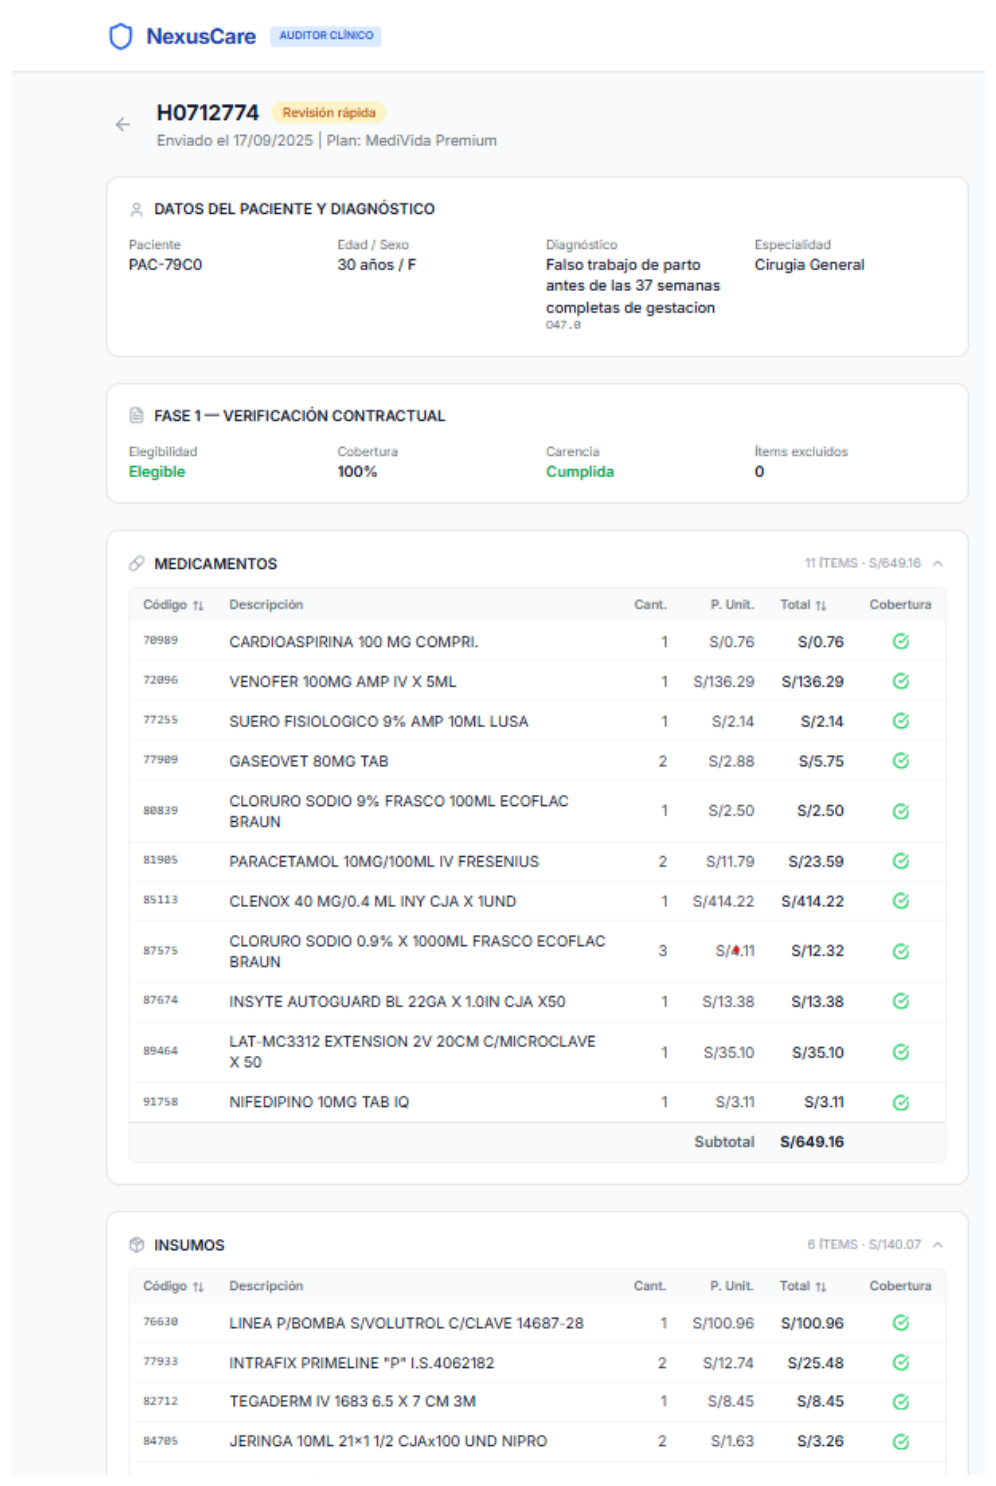
\includegraphics[width=0.96\textwidth,height=0.72\textheight,keepaspectratio]{images/p33_figure_1.png}
\caption{Interfaz del auditor: vista detallada de una liquidación.}
\end{figure}

\section{\textit{Stack} tecnológico}


\begin{table}[H]
    \centering
    \caption{\textit{Stack} tecnológico de NexusCare}
    \label{tab:stack-tecnologico-nexuscare}

    \footnotesize
    \setlength{\tabcolsep}{8pt}
    \renewcommand{\arraystretch}{1.3}

    \begin{tabular}{
        p{0.27\textwidth}
        p{0.65\textwidth}
    }
        \toprule
        \textbf{Capa}
        & \textbf{Tecnología} \\
        \midrule

        \textit{Backend} / \textit{Pipeline}
        & Python 3.11, Pydantic v2, Anthropic SDK y \textit{httpx}. \\

        \textit{Frontend}
        & React 19, TypeScript 5.9, Vite 8, Tailwind CSS 4,
          React Router 7 y \textit{lucide-react}. \\

        Datos
        & JSON (liquidaciones), Parquet (datos crudos) y CIE-10
          (catálogo embebido). \\

        Testing
        & \textit{pytest}, con 190 funciones de prueba distribuidas
          en siete archivos. \\

        Privacidad
        & AES-256-GCM, PBKDF2 para derivación de claves y UUID v4
          para anonimización. \\

        IA
        & Claude Sonnet 4 para \textit{screening} y Claude Opus 4.6
          para análisis profundo. \\

        Diagramas
        & PlantUML C4 y \textit{python-pptx}. \\

        \bottomrule
    \end{tabular}
\end{table}

\section{Decisiones de diseño y \textit{trade-offs}}

\noindent \textbf{1. Arquitectura de dos fases vs. LLM único} Fase 1 (reglas) + Fase 2 (IA) permite que las verificaciones contractuales sean determinísticas, reproducibles y auditables. El \textit{trade-off} es la complejidad adicional de mantener dos subsistemas sincronizados y las configuraciones de plan actualizadas.

\noindent \textbf{2. Estrategia escalonada de modelos vs. modelo único} La combinación Sonnet (\textit{screening}) + Opus (análisis profundo) reduce el costo en un 57 \% respecto a usar Opus en todos los casos, con una pérdida marginal en la profundidad de análisis en los casos de bajo riesgo. El \textit{trade-off} radica en la complejidad de la lógica de escalación.

\noindent \textbf{3. Extracción de reglas de plan mediante LLM + validación humana} Los contratos de seguro son documentos PDF complejos, con lenguaje legal y estructuras variadas entre los planes. La extracción automatizada mediante LLM reduce el tiempo de configuración de días a horas, pero requiere validación humana para garantizar la precisión.

\noindent \textbf{4. \textit{Human-in-the-loop} obligatorio} El sistema nunca toma la decisión final en casos de riesgo medio o alto. La contrapartida es clara: la ganancia de eficiencia queda acotada al segmento de bajo riesgo.

\noindent \textbf{5. \textit{Privacy} by design: PII nunca llega al LLM} Los datos personales se anonimizan antes de enviar cualquier información al modelo y se reidentifican únicamente en el entorno local del auditor, con control de acceso y registro de auditoría.

\section{Resultados preliminares y proyecciones}
\label{sec:resultados-preliminares}

Los resultados del benchmark y las pruebas con el pipeline integrado permiten estimar el desempeño proyectado del sistema en producción.

\textbf{Cobertura de procesamiento} El pipeline procesó exitosamente las 101 liquidaciones del \textit{dataset}  sin errores fatales. La validación estructural con Pydantic v2 no rechazó ningún caso. Los 190 \textit{tests} automatizados cubren el motor de reglas, el pipeline integrado, la lógica de escalación, el \textit{vault} de identidad, el \textit{Golden Set} y la integración \textit{end-to-end}.

\textbf{Distribución de decisiones proyectada} Con los umbrales calibrados y el pre-filtrado de Fase 1, la distribución proyectada para un lote típico de 101 liquidaciones hospitalarias es:

\begin{table}[H]
    \centering
    \caption{Distribución proyectada de decisiones por categoría}
    \label{tab:distribucion-proyectada-decisiones}

    \footnotesize
    \setlength{\tabcolsep}{7pt}
    \renewcommand{\arraystretch}{1.25}

    \begin{tabular}{
        p{0.30\textwidth}
        p{0.18\textwidth}
        p{0.44\textwidth}
    }
        \toprule
        \textbf{Categoría}
        & \textbf{\% proyectado}
        & \textbf{Tiempo estimado de auditoría} \\
        \midrule

        \texttt{FAST\_TRACK}
        & 55--65\,\%
        & $\sim 1$ minuto de verificación visual por caso. \\

        \texttt{REVISION\_RAPIDA}
        & 15--20\,\%
        & $\sim 10$ minutos por caso (revisión focalizada). \\

        \texttt{AUDITORIA\_COMPLETA}
        & 10--15\,\%
        & $\sim 45$ minutos por caso (auditoría profunda). \\

        \texttt{RECHAZO\_ADMINISTRATIVO}
        & 3--5\,\%
        & $\sim 2$ minutos por caso (verificación administrativa). \\

        \bottomrule
    \end{tabular}
\end{table}
Con estos números, el tiempo total del lote se proyecta en 16 horas frente a las 75.8 horas del proceso manual, una reducción del 79 \%.

\textbf{Estimación de costos operativos} El costo de API por lote de 101 liquidaciones, con la estrategia escalonada, fue de \$12.00. Es menos del 0.01 \% del valor promedio de un lote hospitalario.

\textbf{Limitaciones observadas} La principal limitación identificada es la tendencia del LLM a generar hallazgos sobre inconsistencias documentales que pueden ser normales en el flujo operativo de la IPRESS pero que el modelo interpreta como señales de riesgo. Otra limitación es la dependencia de APIs externas para el componente de Fase 2.
